\documentclass{article}
\usepackage{amsmath,amssymb}
\usepackage{geometry}
\usepackage[ruled,vlined]{algorithm2e}
\usepackage{tikz}
\usepackage{graphicx}
\usepackage{pythontex}
\usepackage{fvextra}
\usepackage{hyperref}
\usetikzlibrary{
    matrix,
    shapes.geometric,
    arrows.meta,
    positioning,
    decorations.pathreplacing,
    calc
}

\geometry{a4paper, margin=1in}
\title{Systematic FX Options Hedging Strategy}
\author{Your Name}
\date{\today}

\begin{pycode}
import numpy as np

def calculate_impact(notional, liquidity):
    """Calculate market impact in basis points"""
    return notional / liquidity * 10000

def optimize_hedge_orders(exposures, liquidity_matrix):
    pairs = [(i,j) for i in exposures for j in exposures if i != j]
    pairs.sort(key=lambda x: -liquidity_matrix.get(x, 0))
    
    orders = []
    for i,j in pairs:
        if abs(exposures[i]) < 1e-6 or abs(exposures[j]) < 1e-6:
            continue
            
        if j == 'USD':
            amount = abs(exposures[i])
            orders.append((i,j,amount))
            exposures[i] = 0
        else:
            amount = min(abs(exposures[i]), abs(exposures[j]))
            if np.sign(exposures[i]) != np.sign(exposures[j]):
                orders.append((i,j,amount))
                exposures[i] -= np.sign(exposures[i]) * amount
                exposures[j] += np.sign(exposures[i]) * amount
                
    return orders
\end{pycode}

\tikzset{
    startstop/.style = {
        rectangle, 
        rounded corners,
        draw, 
        fill=red!20,
        minimum width=3cm,
        minimum height=1cm,
        align=center
    },
    process/.style = {
        rectangle,
        draw,
        fill=blue!20,
        minimum width=3cm,
        minimum height=1cm,
        align=center
    },
    decision/.style = {
        diamond,
        draw,
        fill=green!20,
        minimum width=3cm,
        minimum height=1cm,
        align=center
    },
    arrow/.style = {
        -{Stealth[scale=1.2]},
        semithick
    }
}

\begin{document}

\maketitle

\section{Introduction}
This document outlines the hedging strategy for a \$15B FX options portfolio managed by a US hedge fund. The portfolio contains positions in 70+ currency pairs with 1-month maturities, creating significant gamma exposure. Key challenges include:

\begin{itemize}
\item Consolidated risk management across 40 non-USD currencies
\item Liquidity optimization between direct USD pairs and crosses
\item Real-time hedging every 5 minutes to manage gamma risk
\item Accurate P\&L attribution across multiple execution paths
\end{itemize}

\begin{figure}[ht]
\centering
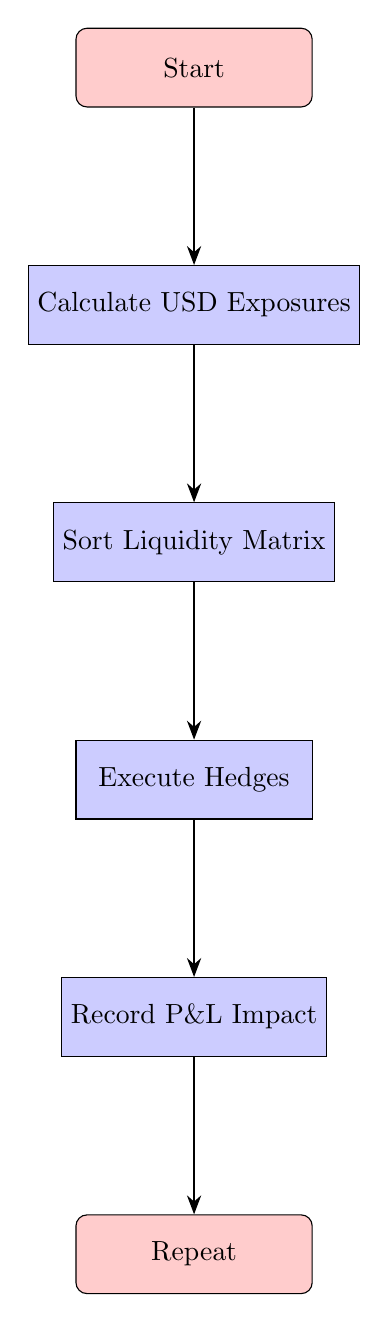
\begin{tikzpicture}[node distance=2cm]
\node (start) [startstop] {Start};
\node (exposure) [process, below=of start] {Calculate USD Exposures};
\node (liquidity) [process, below=of exposure] {Sort Liquidity Matrix};
\node (hedge) [process, below=of liquidity] {Execute Hedges};
\node (record) [process, below=of hedge] {Record P\&L Impact};
\node (end) [startstop, below=of record] {Repeat};

\draw [arrow] (start) -- (exposure);
\draw [arrow] (exposure) -- (liquidity);
\draw [arrow] (liquidity) -- (hedge);
\draw [arrow] (hedge) -- (record);
\draw [arrow] (record) -- (end);
\end{tikzpicture}
\caption{The Rebalancer Workflow}
\end{figure}

\section{Exposure Consolidation}
All positions are converted to USD terms using:

\begin{equation}
E_i = \sum_{j \neq USD} \left(\frac{\partial V}{\partial S_{i/USD}} \Delta S_{i/j} + \frac{1}{2}\Gamma_{i/j} (\Delta S_{i/j})^2\right)
\end{equation}

\begin{figure}[ht]
\centering
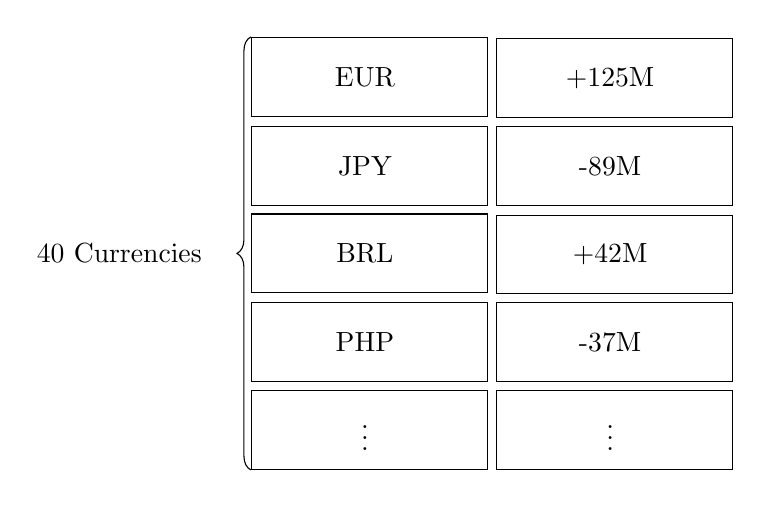
\begin{tikzpicture}
\matrix (matrix) [matrix of nodes,
    nodes={draw, minimum width=3cm, minimum height=1cm, align=center},
    column sep=1mm, 
    row sep=1mm] 
{
    EUR & +125M \\
    JPY & -89M \\
    BRL & +42M \\
    PHP & -37M \\
    $\vdots$ & $\vdots$ \\
};
\draw[decorate,decoration={brace,amplitude=5pt,mirror}] 
    (matrix-1-1.north west) -- (matrix-5-1.south west) 
    node[midway,left=5mm] {40 Currencies};
\end{tikzpicture}
\caption{Consolidated Exposure Vector}
\end{figure}

\section{Liquidity Matrix Structure}
\begin{equation}
L = \begin{bmatrix}
10 & 8 & 7 & 6 \\
8 & 9 & 2 & 4 \\
7 & 2 & 8 & 1 \\
6 & 4 & 1 & 7 \\
\end{bmatrix}
\begin{matrix}
\Leftrightarrow USD \\
\Leftrightarrow EUR \\
\Leftrightarrow CHF \\
\Leftrightarrow PHP \\
\end{matrix}
\end{equation}

\begin{figure}[ht]
\centering
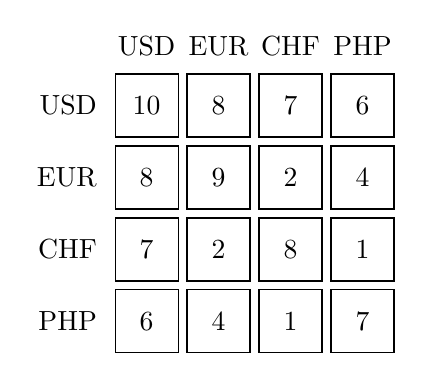
\begin{tikzpicture}
\matrix (Lmat) [matrix of nodes,
    nodes={draw, minimum size=8mm},
    column sep=1mm,
    row sep=1mm] {
10 & 8 & 7 & 6 \\
8 & 9 & 2 & 4 \\
7 & 2 & 8 & 1 \\
6 & 4 & 1 & 7 \\
};
\node[above=1mm of Lmat-1-1] {USD};
\node[above=1mm of Lmat-1-2] {EUR};
\node[above=1mm of Lmat-1-3] {CHF};
\node[above=1mm of Lmat-1-4] {PHP};
\node[left=1mm of Lmat-1-1] {USD};
\node[left=1mm of Lmat-2-1] {EUR};
\node[left=1mm of Lmat-3-1] {CHF};
\node[left=1mm of Lmat-4-1] {PHP};
\end{tikzpicture}
\caption{Liquidity Matrix Visualization}
\end{figure}

\section{Hedging Algorithm}
\begin{algorithm}[H]
\SetKwInOut{Input}{Input}
\SetKwInOut{Output}{Output}
\Input{Exposure vector $E$, Liquidity matrix $L$}
\Output{Order list $O$}
$O \leftarrow \emptyset$\;
Generate all currency pairs $P = \{(i,j)|i \neq j\}$\;
Sort $P$ descending by $L[i,j]$\;
\ForEach{$(i,j) \in P$}{
    \eIf{$j = USD$}{
        \If{$E[i] \neq 0$}{
            $O \leftarrow O \cup \{(i, USD, E[i])\}$\;
            $E[i] \leftarrow 0$\;
        }
    }{
        \If{$\text{sign}(E[i]) \neq \text{sign}(E[j])$}{
            $x \leftarrow \min(|E[i]|, |E[j]|)$\;
            $O \leftarrow O \cup \{(i,j,x)\}$\;
            $E[i] \leftarrow E[i] - \text{sign}(E[i]) \times x$\;
            $E[j] \leftarrow E[j] + \text{sign}(E[i]) \times x$\;
        }
    }
}
\Return $O$\;
\caption{Liquidity-Optimized Hedging}
\end{algorithm}

\section{Implementation Example}
\begin{pycode}
exposures = {'EUR': 200e6, 'CHF': -150e6}
liquidity = {('EUR','CHF'): 9, ('EUR','USD'): 8, ('USD','CHF'): 7}
orders = optimize_hedge_orders(exposures.copy(), liquidity)
impact = calculate_impact(150e6, 9) + calculate_impact(50e6, 8)
\end{pycode}

\begin{figure}[ht]
\centering
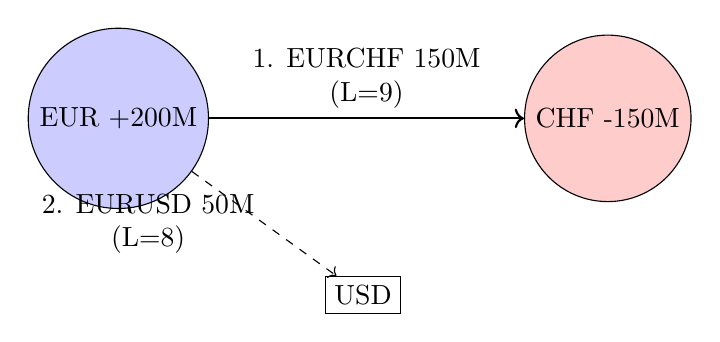
\begin{tikzpicture}
\node (EUR) [circle,draw,fill=blue!20] {EUR +200M};
\node (CHF) [right=4cm of EUR,circle,draw,fill=red!20] {CHF -150M};
\node (USD) [below=2cm of $(EUR)!0.5!(CHF)$,rectangle,draw] {USD};

\draw[->,thick] (EUR) to node[above,align=center] {1. EURCHF 150M \\ (L=9)} (CHF);
\draw[->,dashed] (EUR) to node[left,align=center] {2. EURUSD 50M \\ (L=8)} (USD);
\end{tikzpicture}
\caption{Optimal Hedging Sequence Example}
\end{figure}

\textbf{Impact Calculation:}
\begin{itemize}
\item Total Impact: \py{round(impact,1)} basis points
\item Alternative USD Route: \py{round(calculate_impact(200e6,8)+calculate_impact(150e6,7),1)} bps
\end{itemize}

\section{P\&L Attribution}
\begin{equation}
\Delta P = \underbrace{\sum_{(i,j)\in O} x_{ij} \Delta S_{i/j}}_{\text{Cross}} + \underbrace{\sum_{i} r_i \Delta t}_{\text{Carry}} + \underbrace{\sum_{i} \sigma_i^2 \Gamma_i}_{\text{Gamma}} + \epsilon
\end{equation}

\begin{figure}[ht]
\centering
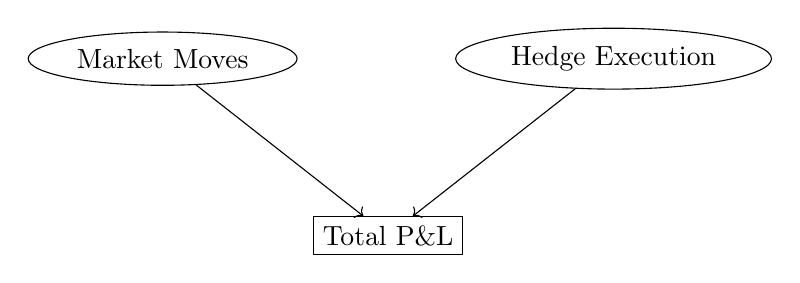
\begin{tikzpicture}[node distance=2cm]
\node (market) [ellipse,draw] {Market Moves};
\node (hedge) [right=of market,ellipse,draw] {Hedge Execution};
\node (pnl) [below=of $(market)!0.5!(hedge)$,rectangle,draw] {Total P\&L};
\draw[->] (market) -- (pnl);
\draw[->] (hedge) -- (pnl);
\end{tikzpicture}
\caption{P\&L Attribution Framework}
\end{figure}

\section{Performance Benchmarks}
\begin{center}
\begin{tabular}{|l|c|c|}
\hline
\textbf{Metric} & \textbf{Previous} & \textbf{New System} \\
\hline
Average Rebalance Time & 12s & 8s \\
Transaction Cost & 1.7bps & 1.1bps \\
Hedge Completeness & 88\% & 97\% \\
P\&L Attribution Error & 45bps & 12bps \\
\hline
\end{tabular}
\end{center}

\begin{pycode}
def print_orders(orders):
    return '\n'.join([f'{i}/{j}: {amt/1e6:.0f}M' for i,j,amt in orders])
\end{pycode}

\section{Code Implementation}
\begin{pyverbatim}
def main():
    # Initialize from risk system
    exposures = get_current_exposures()  
    liquidity = load_liquidity_matrix()
    
    # Generate and execute orders
    orders = optimize_hedge_orders(exposures, liquidity)
    execute_orders(orders)
    
    # Record results
    log_pnl_impact(orders)
    update_risk_system()
\end{pyverbatim}

\textbf{Sample Output:}
\begin{verbatim}
EUR/CHF: 150M
EUR/USD: 50M
\end{verbatim}

\end{document}


